\section{General Architecture \& Code Generation}
\label{sec:CG}

Fundamentally, \IOTDSL describes a real-time reactive system: information is regularly reported to the middleware where it is processed in order to react back on the environment. However, in the context of \IOT systems, the environment cannot be controlled, but it is perceived through the many deployed devices, that allow at the same time to react on it. The key task is then to process events quickly enough to ensure appropriate reactions, although it it not critical to react in a precise timeframe. In this section, we first describe the general architecture of our tool as well as the technical choices for processing events in an \IOT system, then provide a compilation schema to translate \IOTDSL business rules into Tesla rules, the entry language of TRex \cite{cugola-12}, the \CEP engine we have chosen in our architecture.

\subsection{General Architecture}
\label{sec:CG-Architecture}

Our proposal relies on a middleware that embeds a \CEP engine for handling event processing, as depicted in Figure \ref{fig:Architecture}. Our tool offers a simulation mode, where devices are simulated as software components mimicking their actual execution, thus allowing to test \IOT scenarios without physical devices.

\begin{figure}%
	\centering  
	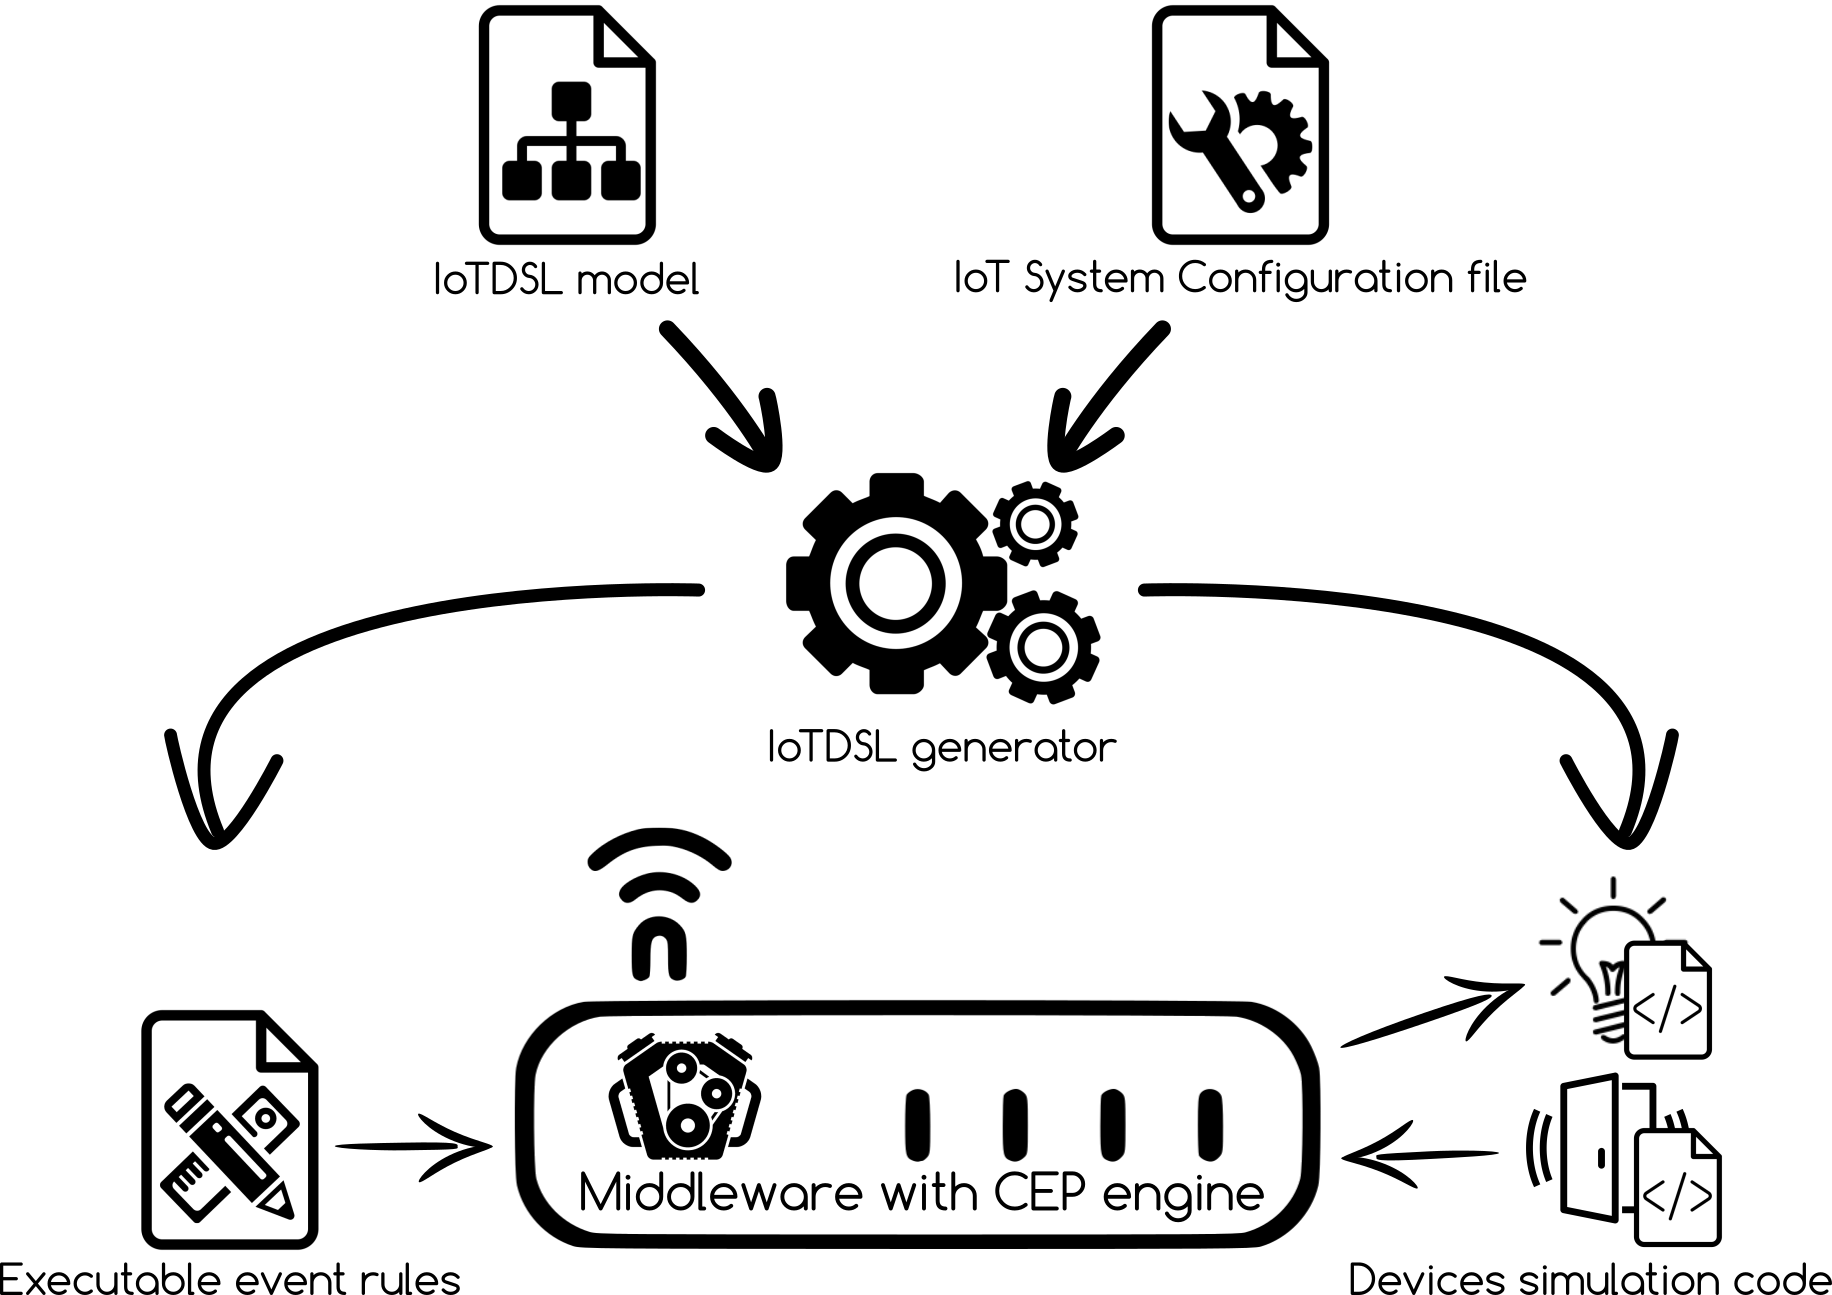
\includegraphics[width=.9\linewidth]{gen-archi.png}%
	\caption{General architecture of \IOTDSL framework}%
	\label{fig:Architecture}%
\end{figure}

The central element is the automatic code generator process: it produces executable code from \IOTDSL models and configuration files that define platform-specific details on the execution timing of devices (that the technicians set once and for all), and, for the purpose of our prototype, simulation code used to emulate the behaviour of the devices. The executable code is deployed into the \CEP engine running on a middleware, which reuses in simulation mode the simulation code for communicating with the (abstract) devices. 

%From \IOTDSL models, the generator will create a set of files that gather, on the one side, all rules as executable complex events and on the other side, a set of simulation code used to emulate the devices' behaviours. The event rules will be deployed in a \CEP engine running on a middleware and the individual simulation files will be used to test the whole infrastructure.

We are currently investigating how business rules could be broken down into smaller clusters that could be deployed directly into devices, assuming they present sufficient battery and computing power. When addressing non-functional properties of devices, we envision the possibility of expressing technical specifications relative to the energy consumption and computation capabilities of devices in a separate file that \IOTDSL would take into consideration for identifying distributable rules.

%As we already mentioned, at present time the rules are all gathered and managed by a centralised entity where the simulation files are each emulating a single device. We are currently investigating how all business rules can be split into smaller chunks to be run on devices themselves when those objects have sufficient battery and CPU power. As we are developing the non-functional properties for \IOTDSL type and mapping definitions, those characteristics will be expressible in the form of technical specifications for devices and thus powerful equipments that are meeting some minimum requirements will be identified as deployment targets for distributed \CEP engines. 
\subsection{TRex as \CEP engine}
\label{sec:CG-TRex}

To enable efficient event processing from distributed connected things, we rely on TRex, a powerful and highly optimised \CEP engine developed by Cugola and Margara~\cite{cugola-12}. TRex relies on Tesla \cite{Cugola-Margara:2010}, an entry language that is expressive enough to address most of the necessary patterns for capturing complex events definitions. As a consequence, the expression language used for \IOTDSL \textsc{triggers} is directly inspired from Tesla. This allows us to offer end-users the expressibility they need, while at the same time simplifying the translation of \IOTDSL rules into Tesla rules. 

TRex offers a queueing mechanism to overcome bursts of incoming events: when deploying the \IOT system on site, it becomes possible to customise the queue size, thus balancing between event loss and treatment latency. 

TRex is conveniently organised as a Client/Server architecture in a \textit{<<publish / subscribe>>} way, and relies on the Tesla language to define the necessary components: event \emph{notifications} (or \emph{occurrences}, or simply events); \emph{subscriptions} and \emph{rules}. TRex, as the \CEP engine, permanently receives event notifications from sources, and redistribute them to subscribers. 
An event notification is produced by a source and sent to the \CEP system, and is typed by an event type that possesses typed attributes: for example, \inlineT{Temp@100(location = ``Living'', value = 25.0)} defines a notification of type \inlineT{Temp} with two attributes and a timestamp (noted after the \inlineT{@}) that records the moment in time the notification is produced. A subscription by sinks (or, event consumers) is submitted to the \CEP system in order to receive notifications that things happened: for example, \inlineT{Subscribe(Temp, location = ``Living'' and value > 20)} indicates a subscription to \inlineT{Temp} notification that matches the filtering condition on its location and value. Tesla rules define complex events from simpler ones, which may emanate from actual sources, or be complex events defined by other rules, thus leading to a hierarchy of events. 

A rule has the following form:
\begin{lstlisting}[language=tesla, numbers=none]
	define CE(attr1 : Type1, ..., attrN : TypeN)
	from   Pattern
	where  attr1 := f1, ..., attrN := fN
\end{lstlisting}
Intuitively, a rule defines a complex event \inlineT{CE} together with its signature (i.e. an ordered list of typed attributes) that issues \inlineT{CE} notifications whenever the \inlineT{Pattern} is matched, assigning values to \inlineT{CE} attributes from the functions defined in the \inlineT{where} clause (that may depend on elements of the \inlineT{Pattern}). Valid patterns include event \emph{occurrences} that filter attribute values (e.g., \inlineT{from Temp.val > 20}), event \emph{compositions} that combine events together with boolean operators or time windows (e.g., \inlineT{from Rain and Temp.val > 20 within 5 min from Smoke}, indicating that a temperature reading above 20°C should occur within five minutes from a \inlineT{Smoke} notification, while raining); event \emph{negation} (e.g., \inlineT{from not Rain between Temp and Smoke}, indicating that it should not rain between an elevated temperature reading and a smoke notification). Tesla proposes more powerful patterns like aggregation and iterations, but we will not use them in our examples.
Note that the server is interactive so that clients can (un-)subscribe while the engine is running and rules may be added or deleted at runtime without affecting the overall infrastructure. 

From the perspective of \IOTDSL, TRex offers several benefits as a \CEP engine. TRex is powerful enough to handle typical \IOT scenarios like the one described in Section \ref{sec:Motivation}, thanks to the expressive power of Tesla. It adopts a decentralised architecture that directly reflects our design choices, and supports distributed processing of events to reduce the cost of communication and to optimise resource usage. It is developed in C, so it is even suitable for \textit{small form factor} middlewares. Finally, on top of an \textsc{API} written in C, Java libraries have been developed on which we rely to generate devices' simulation code.

\subsection{Compiling \IOTDSL Rules}
\label{sec:CG-Compilation}

We now describe how we obtain the final code deployed into the gateway using TRex, and illustrate our compilation scheme on the Business Rules of Section \ref{sec:IoTDSL-BusinessRules}.

In \IOTDSL, a Business Rule has the following general form: \inlineI{rule R: when (trigger) do reaction}. The scheme for producing Tesla code relies on a three-step process:
\begin{enumerate}
	\item For traceability purposes, we map each rule name \inlineI{R} to the resulting Tesla rule(s), to be able to trace in the future analysis results directly back to \IOTDSL rules.
	
	\item The second step requires a preliminary task: since Tesla does not handle instances (in the form of our dot-like notation for events), we need to add a predefined attribute \inlineT{E(_inst : Instance)} to each event \inlineI{E} used in \IOTDSL Business Rules, and link the type \inlineI{Instance} to simple strings; unicity of instance names is ensured by \IOTDSL while checking Network Configurations. The rest of the second step depends on the nature of the \inlineI{reaction}:
	\begin{itemize}
		\item If it is not a composite, i.e. the rule consists of only one actuation of the form \inlineI{inst.actuation(<param1, ..., paramN>)}, we translate it in a simple rule of the form
		\begin{lstlisting}[language=tesla, numbers=none]
	define actuation(param1, ..., paramN)
	from   transformedTrigger
	where  param1 := f1, ..., paramN := fN
		\end{lstlisting}
		where the actuation parameters are computed in the \inlineT{where} line, and the \inlineI{trigger} condition is transformed into \inlineT{transformedTrigger} with the process in Step 3.
		
		\item If the \inlineI{reaction} is composite, i.e. it consists of several actions \inlineI{a1}, \ldots, \inlineI{aN}, we issue $n+1$ Tesla rules: one rule for each actuation \inlineI{aI}, and one additional rule to bind things together.
		\begin{center}
			\begin{lstlisting}[language=tesla, numbers=none]
	define R(Rparam1, ..., RparamM)
	from   transformedTrigger
	where  Rparam1 := g1, ..., RparamM := gn
	...
	define aI(AIparam1, ..., AIparamN)
	from   R(Rparam1, ..., RparamM)
	where  AIparam1 := f1, ..., AIparamN := fn
	...
			\end{lstlisting}
		\end{center}
		When the event pattern for the rule \inlineI{R} is detected, the first rule issues the complex event \inlineT{R}, which is immediately produced by the \CEP engine to trigger the subsequent rules. This way, all actuations are processed at the same time, leaving the platform handling how to effectively enforce the actuations. Note that in the additional Tesla rule \inlineT{R}, no \inlineT{_inst} parameter appears (as it is not needed), but all parameters necessary to the $n$ actuations are part of event \inlineT{R}'s signature, so that functions \inlineT{f1}, ..., \inlineT{fN} rematches the parameters of each actuation (\inlineI{aIparamK}) correctly from \inlineT{R}'s parameters.
	\end{itemize}
	\item It then remains to compute the \inlineT{transformedTrigger} appearing in Tesla rules, which depends on whether facilitators (like \inlineI{after} or \inlineI{before}) have been used. In the absence of facilitators, the transformation is straigthforward since the same expressions are natively available in Tesla. Otherwise, we rely on an external configuration file that describe the expected latency delays specific to devices and their communication paths, to translate such triggers into appropriate time windows. Producing this file is not the responsibility of the end-user, since it rather leverages knowledge pertaining to the \IOT system installation and deployment. 
\end{enumerate}

Let us now apply this compilation scheme to the three Business Rules described in Section \ref{sec:IoTDSL-BusinessRules}. Rule \inlineI{SwitchBathroomLightOffAtNight} is the simplest one: it contains only one actuation, and its triggers has a regular Tesla time window expression. Applying our compilation scheme results in the following Tesla rule:
\begin{lstlisting}[language=tesla, numbers=none]
	define Off(_inst : Instance)
	from   not Movement(_inst = hallMotion) within 3 min from Closed(_inst = childDoor)
	where  _inst = bathroomBulb
\end{lstlisting}
Note that all event names are capitalised to cope with Tesla entry language, and that the \inlineT{from} clause only binds the \inlineT{_inst} attributes to their respective instances in the source \IOTDSL rule. 

Rule \inlineI{SwitchLightsWhenEntering} is a good illustration of \IOTDSL rules with multiple actuations. Applying the compilation scheme results in three rules, one for each actuation, and an additional one that glues things together. 
\begin{lstlisting}[language=tesla, numbers=none]
	define SwitchLightsWhenEntering
	from   Moving(_inst = foyerMotion) within 10 sec from Opened(_inst = frontDoor)

	define On(_inst : Instance)
	from   SwitchLightsWhenEntering
	where  _inst = foyerBulb
	
	define On(_inst : Instance)
	from   SwitchLightsWhenEntering
	where  _inst = livingBulb
\end{lstlisting}
The additional rule defining the \inlineT{SwitchLightsWhenEntering} event does not define an \inlineT{_inst} attribute, and converts the event facilitator \inlineI{after} into a time window from a predefined value (here, 10 seconds). The two other rules originate from the actuators that have the particularity to activate the same event on two different devices (\inlineI{foyerBulb} and \inlineI{livingBulb}): this results in the same rule with different bindings for \inlineT{_inst}.

Rule \inlineI{SwitchBathroomLightOnAtNight} is the most complicated, since it combines negation outside a time window. Applying the compilation scheme results in only one rule, since there is only one actuation, but the trigger condition is more complicated that the first rule. Since Tesla does not support negation operators outside of time windows, we need to integrate it inside one. Intuitively, the starting point of this scenario is the opening of the door room: at this point, the bathroom light should be switch on if movement is detected shortly after and there is currently no light in the living. Such trigger patterns are detected and refactored as follows: 
\begin{lstlisting}[language=tesla, numbers=none]
	define On(_inst : Instance)
	from   (Light(_inst = livingLight) within  2 sec from Opened(_inst = childDoor)) and 
			   (Moving(_inst = hallMotion) within 10 sec from Opened(_inst = childDoor))
	where  _inst = bathroomBulb
\end{lstlisting}
